\subsection{Tuning of ESKF for real data}
The next step was to see how the error state Kalman filter would perform on actual real life data. The available dataset contains IMU and GNSS measurements of a unmanned aerial vehicle (UAV) remotely controlled by an operator. The flight path of the UAV as seen from the GNSS measurements is shown in figure \ref{fig:real-track}.
\begin{figure}[H]
\centering
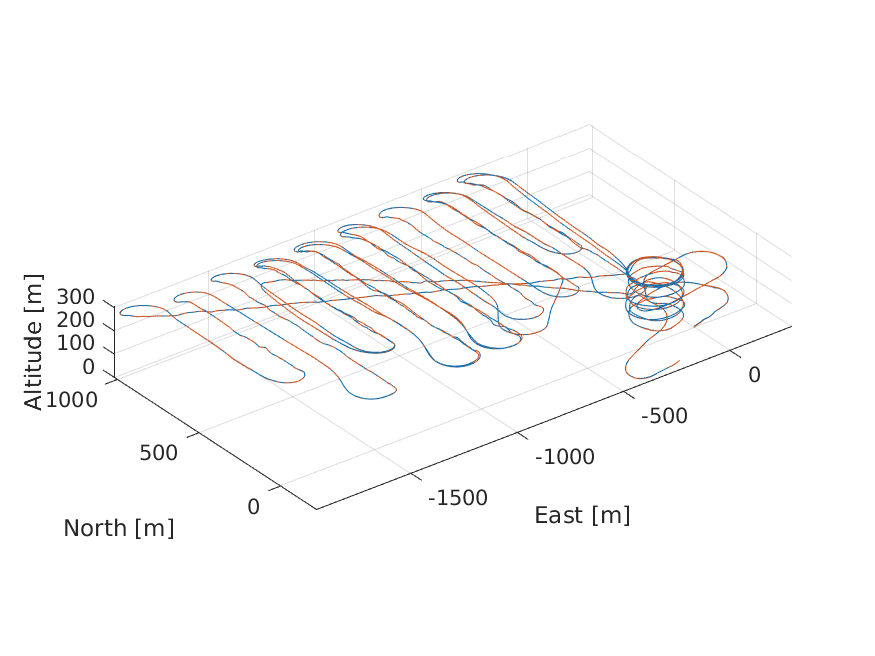
\includegraphics[width=0.6\textwidth]{plots/a2-real-track}
\caption{UAV Track}
\label{fig:real-track}
\end{figure}
With this real dataset, there are some other complications that must be adressed. Firstly is the correction matrices $S_a$ and $S_g$ for the gyro and the accelerometer. These matrices correct for the orientation of the IMU in the body frame of the AUV. They also correct for misaligned axes IMU axes (that is, the IMU may be slightly malproduced with axes that are skewed somewhat off the orthogonal coordinate axes). These matrices however are of course not known exactly, because they are supposed to correct for unknown manufacturing errors, for this reason must expect some inaccuracy in the measurements. The second complication is the leverarm. This is the distance between the cener of control on the AUV and the mounting position of the IMU. This value has been measured and is given in the dataset. We give it as an input to the ESKF.

The tuning of the kalman filter is again based on the STIM300 datasheet, as this is the actual IMU used on the UAV. In this case, we do not have the ground truth available, so we cannot calculate the normalised error state squared (NEES), we can however use the \textit{innovation} of the kalman filter, which in layman terms is a measure of how much the filter must update or "innovate" the estimate in the update step to correct for the new measurement, in other words a measure of how "off" the prediction is. With our tuning, we are able to achieve a normalized innovation squared (NIS) that stays $80\%$ inside the $95\%$ $\chi^2$ confidence interval, shown in figure \ref{fig:nis_basic} below.
\begin{figure}[H]
        \centering
        \begin{subfigure}[b]{0.45\textwidth}
                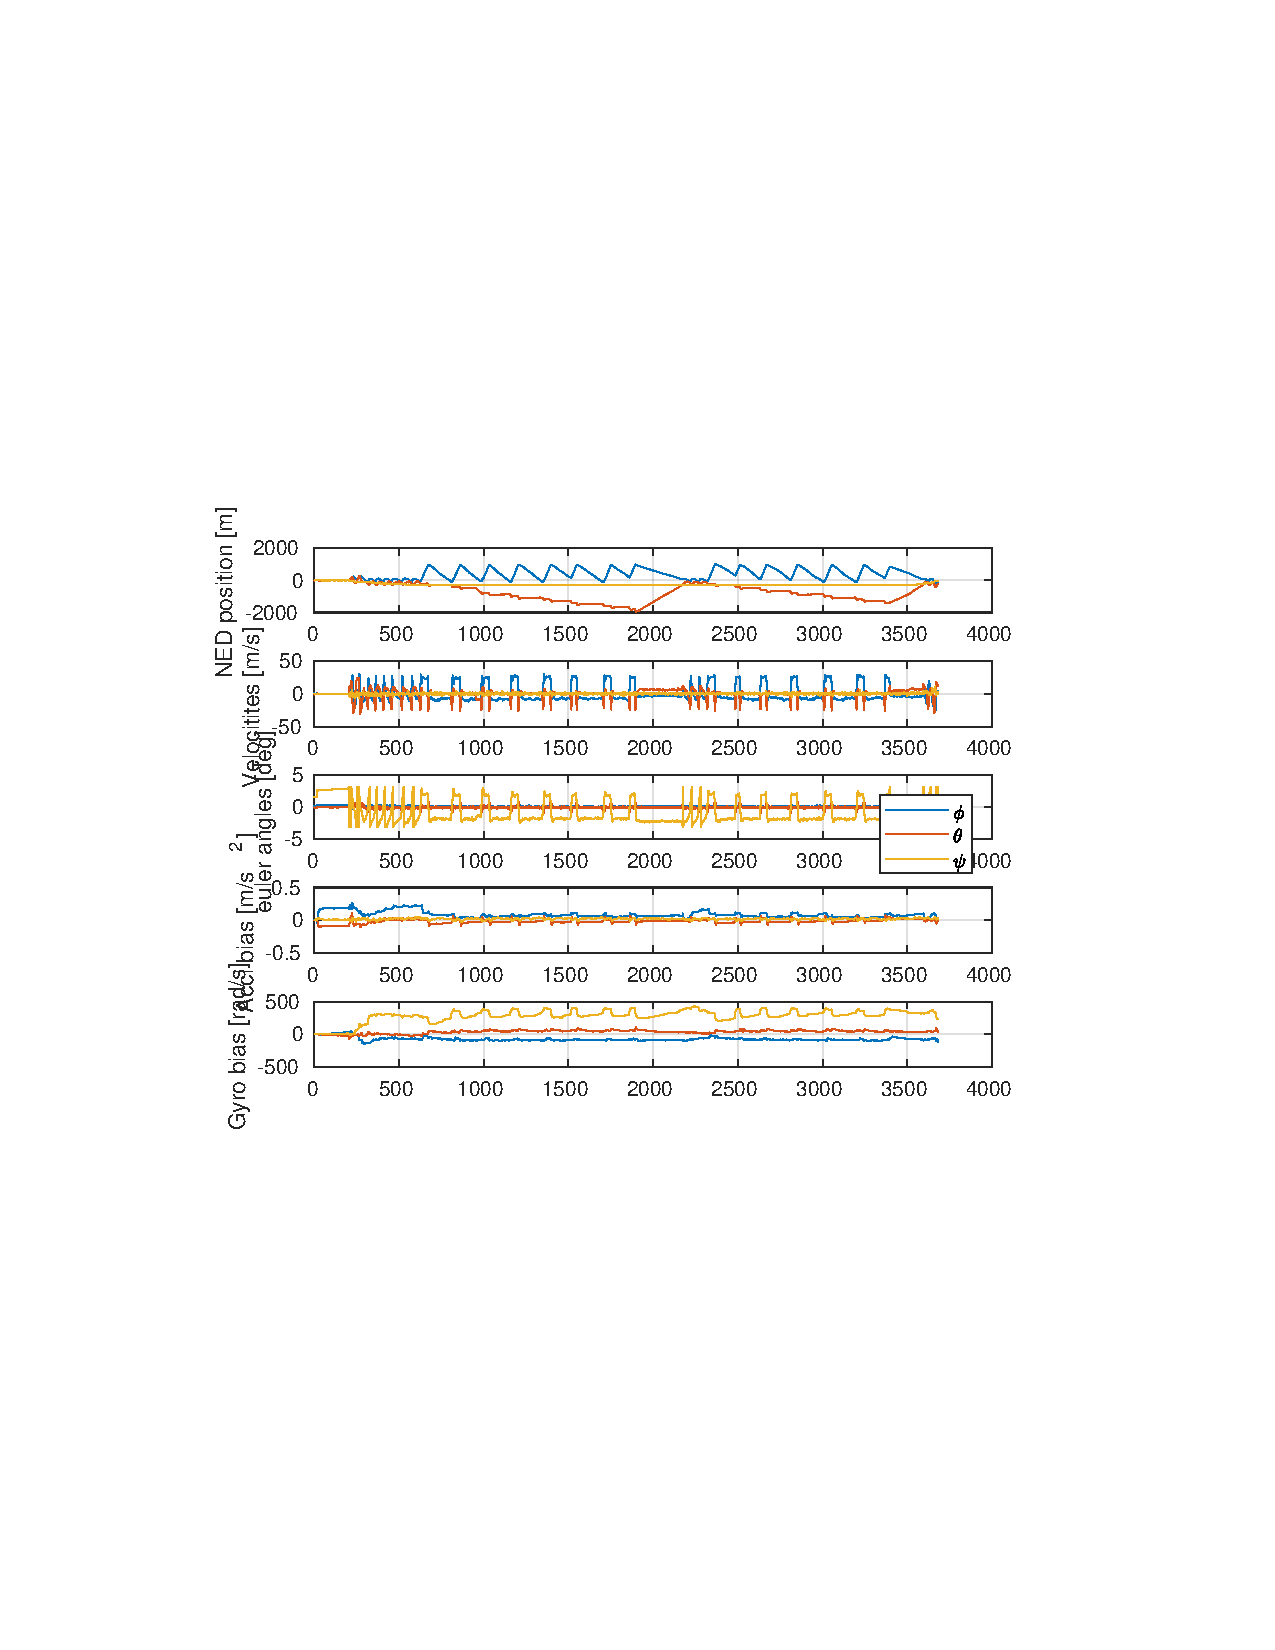
\includegraphics[width=\textwidth]{plots/a2-real-nis}
                \caption{NIS }
                \label{fig:nis_basic}
        \end{subfigure}%
~
        \begin{subfigure}[b]{0.45\textwidth}
                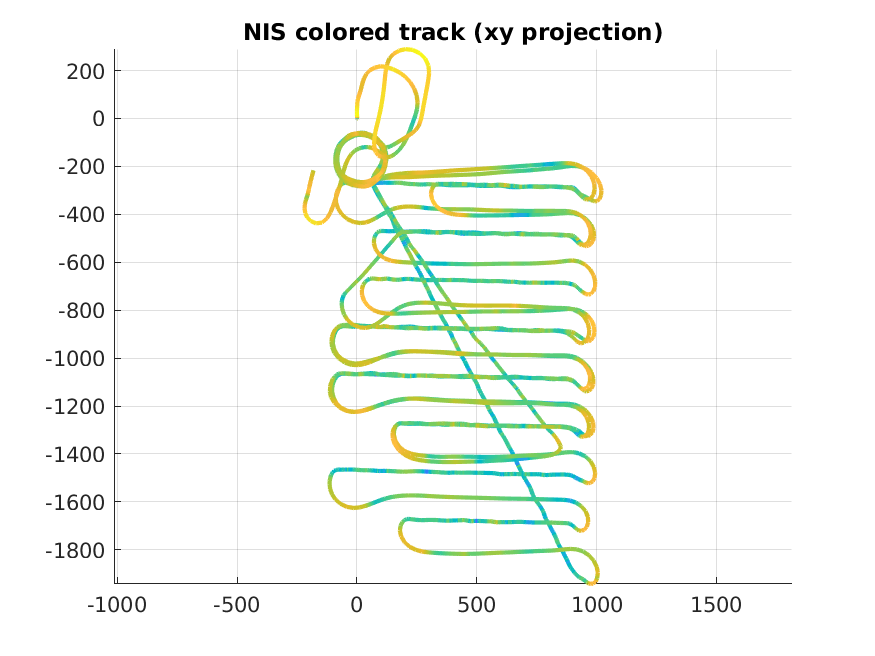
\includegraphics[width=\textwidth]{plots/a2-real-nis-colored-track}
                \caption{NIS colored track}
                \label{fig:nis_colored_track}
        \end{subfigure}
        \caption{Normalized Innovation Squared}
        \label{fig:nis}
\end{figure}
Interisting to note about the NIS, are the seemingly periodic spikes that leave the confidence interval. By superimposing the NIS value over the 2D-projected AUV trajectory, like shown in figure \ref{fig:nis_colored_track}, it is evident that the spikes appear when the AUV is turning. This stems from the fact that turns are non-linear motion, and the ESKF uses a linearization model. We also note the large spike in NIS early in figure \ref{fig:nis_basic}. This spike appears at $t=206s$, right as the AUV is catapulted into the air, as such it is natural to expect a large innovation value.
